\documentclass[12pt]{article}
\usepackage{geometry}
\geometry{a4paper, total={170mm, 250mm}}
\title{\textbf{Homework 6}}
\author{Maedeh Karkhane Yousefi}
\usepackage{float}
\usepackage{graphicx}
\usepackage{amsmath}
\usepackage{amssymb}
\usepackage{subcaption}
\usepackage{hyperref}
\hypersetup{
    colorlinks=true,
    linkcolor=blue,
    filecolor=magenta,      
    urlcolor=cyan,
    }
\begin{document}
\maketitle
\part*{1. Exercise 7.1: SS MC and IS MC}
\paragraph*{}
The absolute answer is:
\begin{center}
$I= \int_{0}^2 e^{-x^2}= \sqrt{\pi}/2\ erf(2)$
\end{center}
ISMC:\\
We calculate the integral knowing the function $g(x)= e^{-x}$, and the integral is $\int_{0}^2 e^{-x^2}$. The exact answer is:
\begin{center}
$\int_{0}^2 e^{-x^2}= 1-e^{-2}$\\
$y=-ln(1-x(1-e^{-2}))$
\end{center}
\begin{figure}[H]
	\centering
	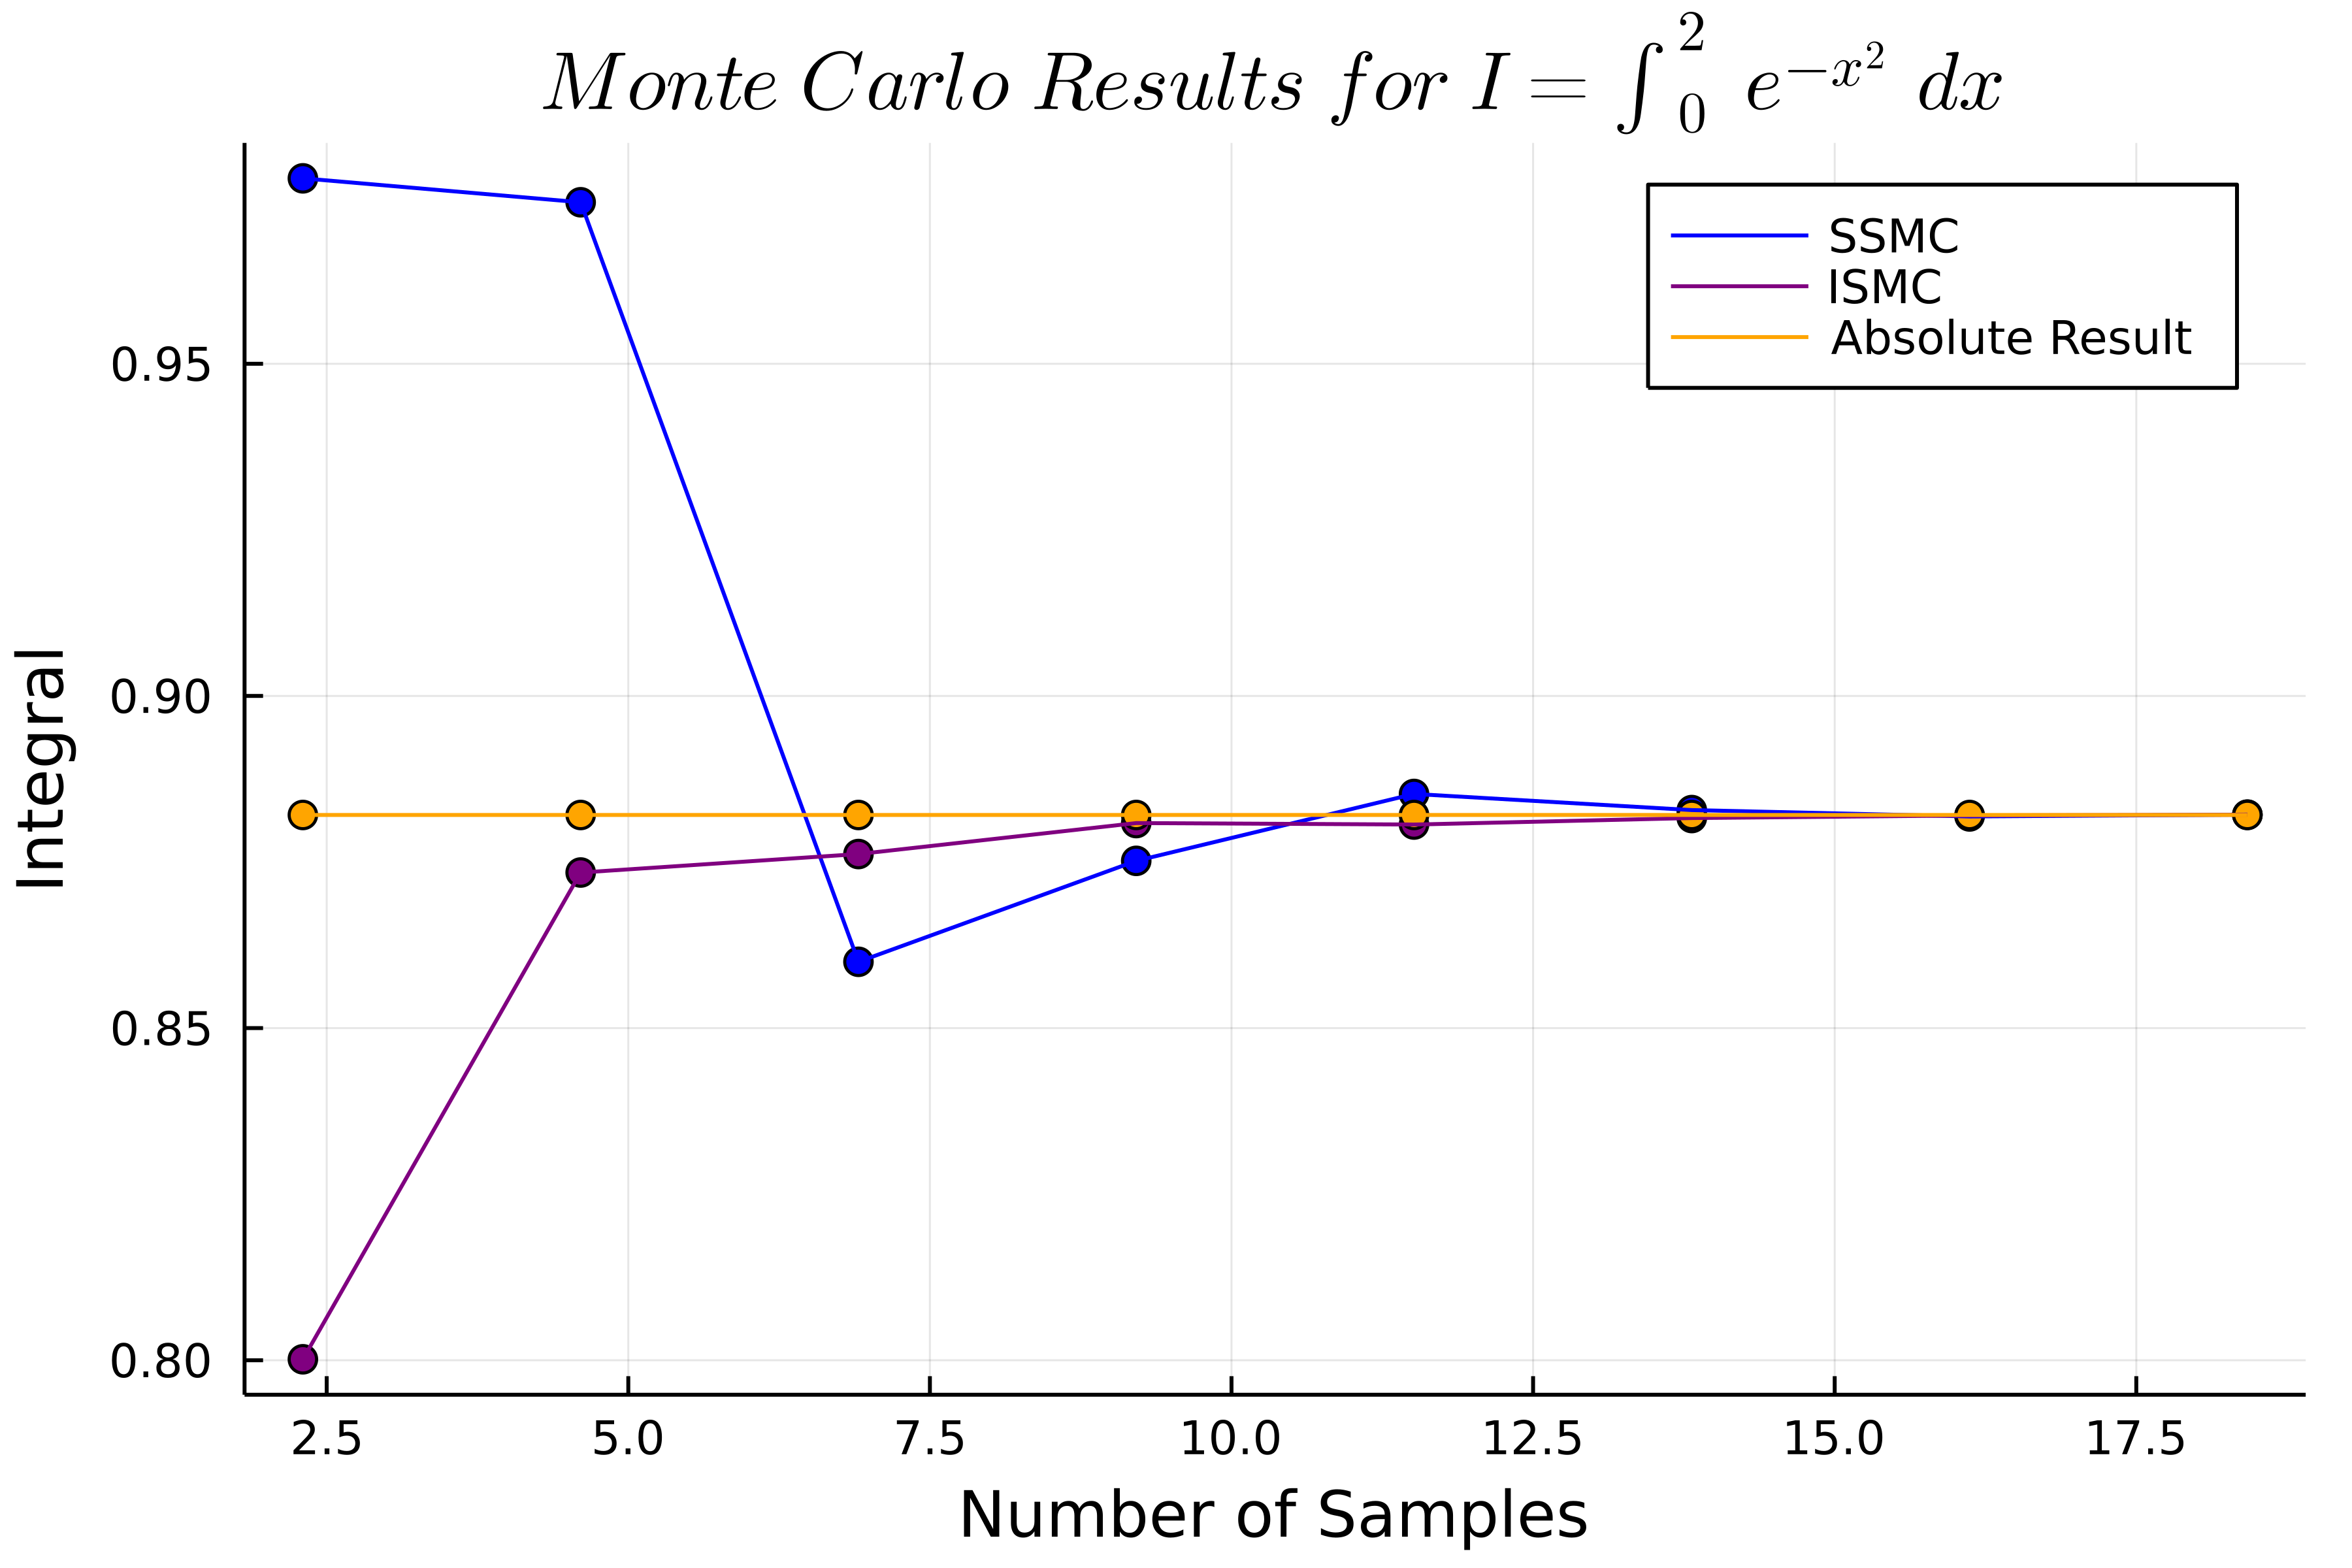
\includegraphics[width=\textwidth]{ResultsPlot.png}
	\label{fig:mesh1}
	\caption{The Answers for 8 samples using SSMC and ISMC method. samples are between $10^{1}$ to $10^{8}$ multiplying by 10 each step.}
\end{figure}
\begin{figure}[H]
	\centering
	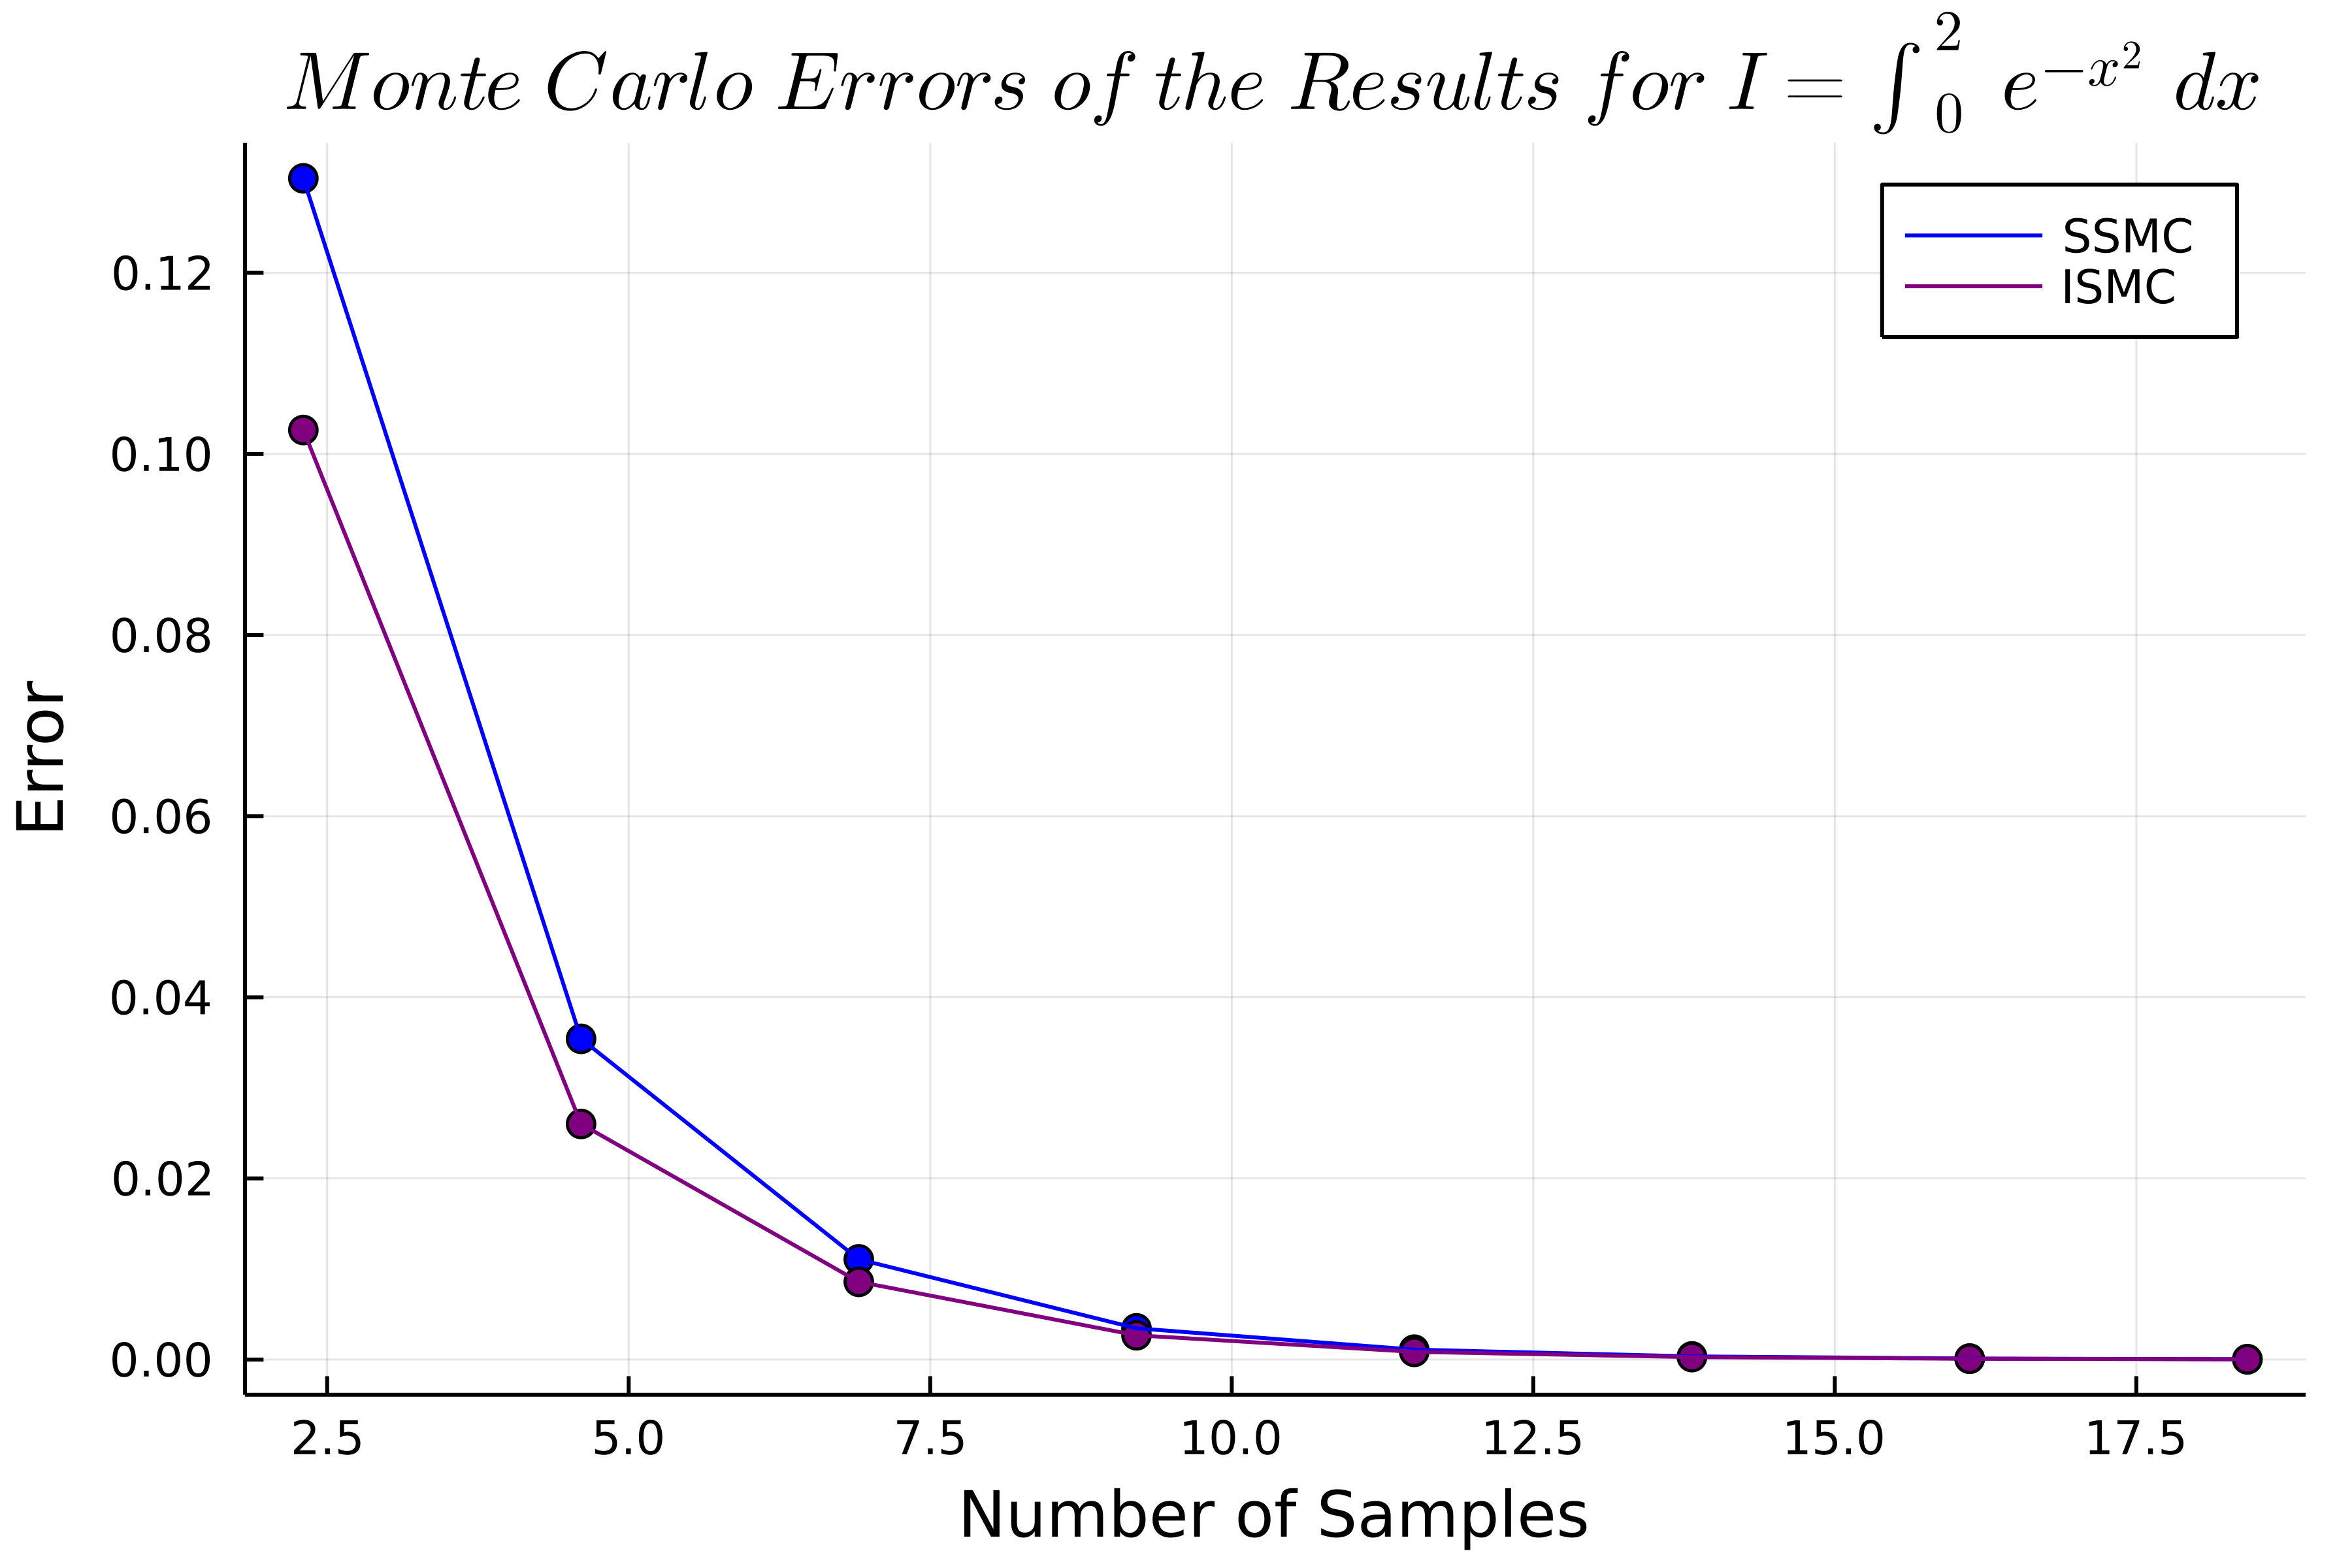
\includegraphics[width=\textwidth]{ErrorPlot.png}
	\label{fig:mesh1}
	\caption{The errors of the answers for 8 samples using SSMC and ISMC method. samples are between $10^{1}$ to $10^{8}$ multiplying by 10 each step.}
\end{figure}
\part*{2. Exercise 7.2}
\paragraph*{}
Using 2D Integration, I tried to find the center of mass of the sphere wanted in the textbook. knowing that: 
\begin{center}
$R_{CoM} = \frac{I}{M}$\\
$ R_{CoM} = \frac{\int_0^R\int_0^\pi (3+\frac{r}{R}\cos{\theta})r^3\sin{\theta}\cos{\theta} d\theta dr}{\int_0^R\int_0^\pi (3+\frac{r}{R}\cos{\theta})r^2\sin{\theta} d\theta dr}$\\
\end{center}
The exact answer is: R/15 (assuming R=1, the answer is 1/15).
\begin{figure}[H]
	\centering
	\begin{subfigure}[t]{0.8\textwidth}
		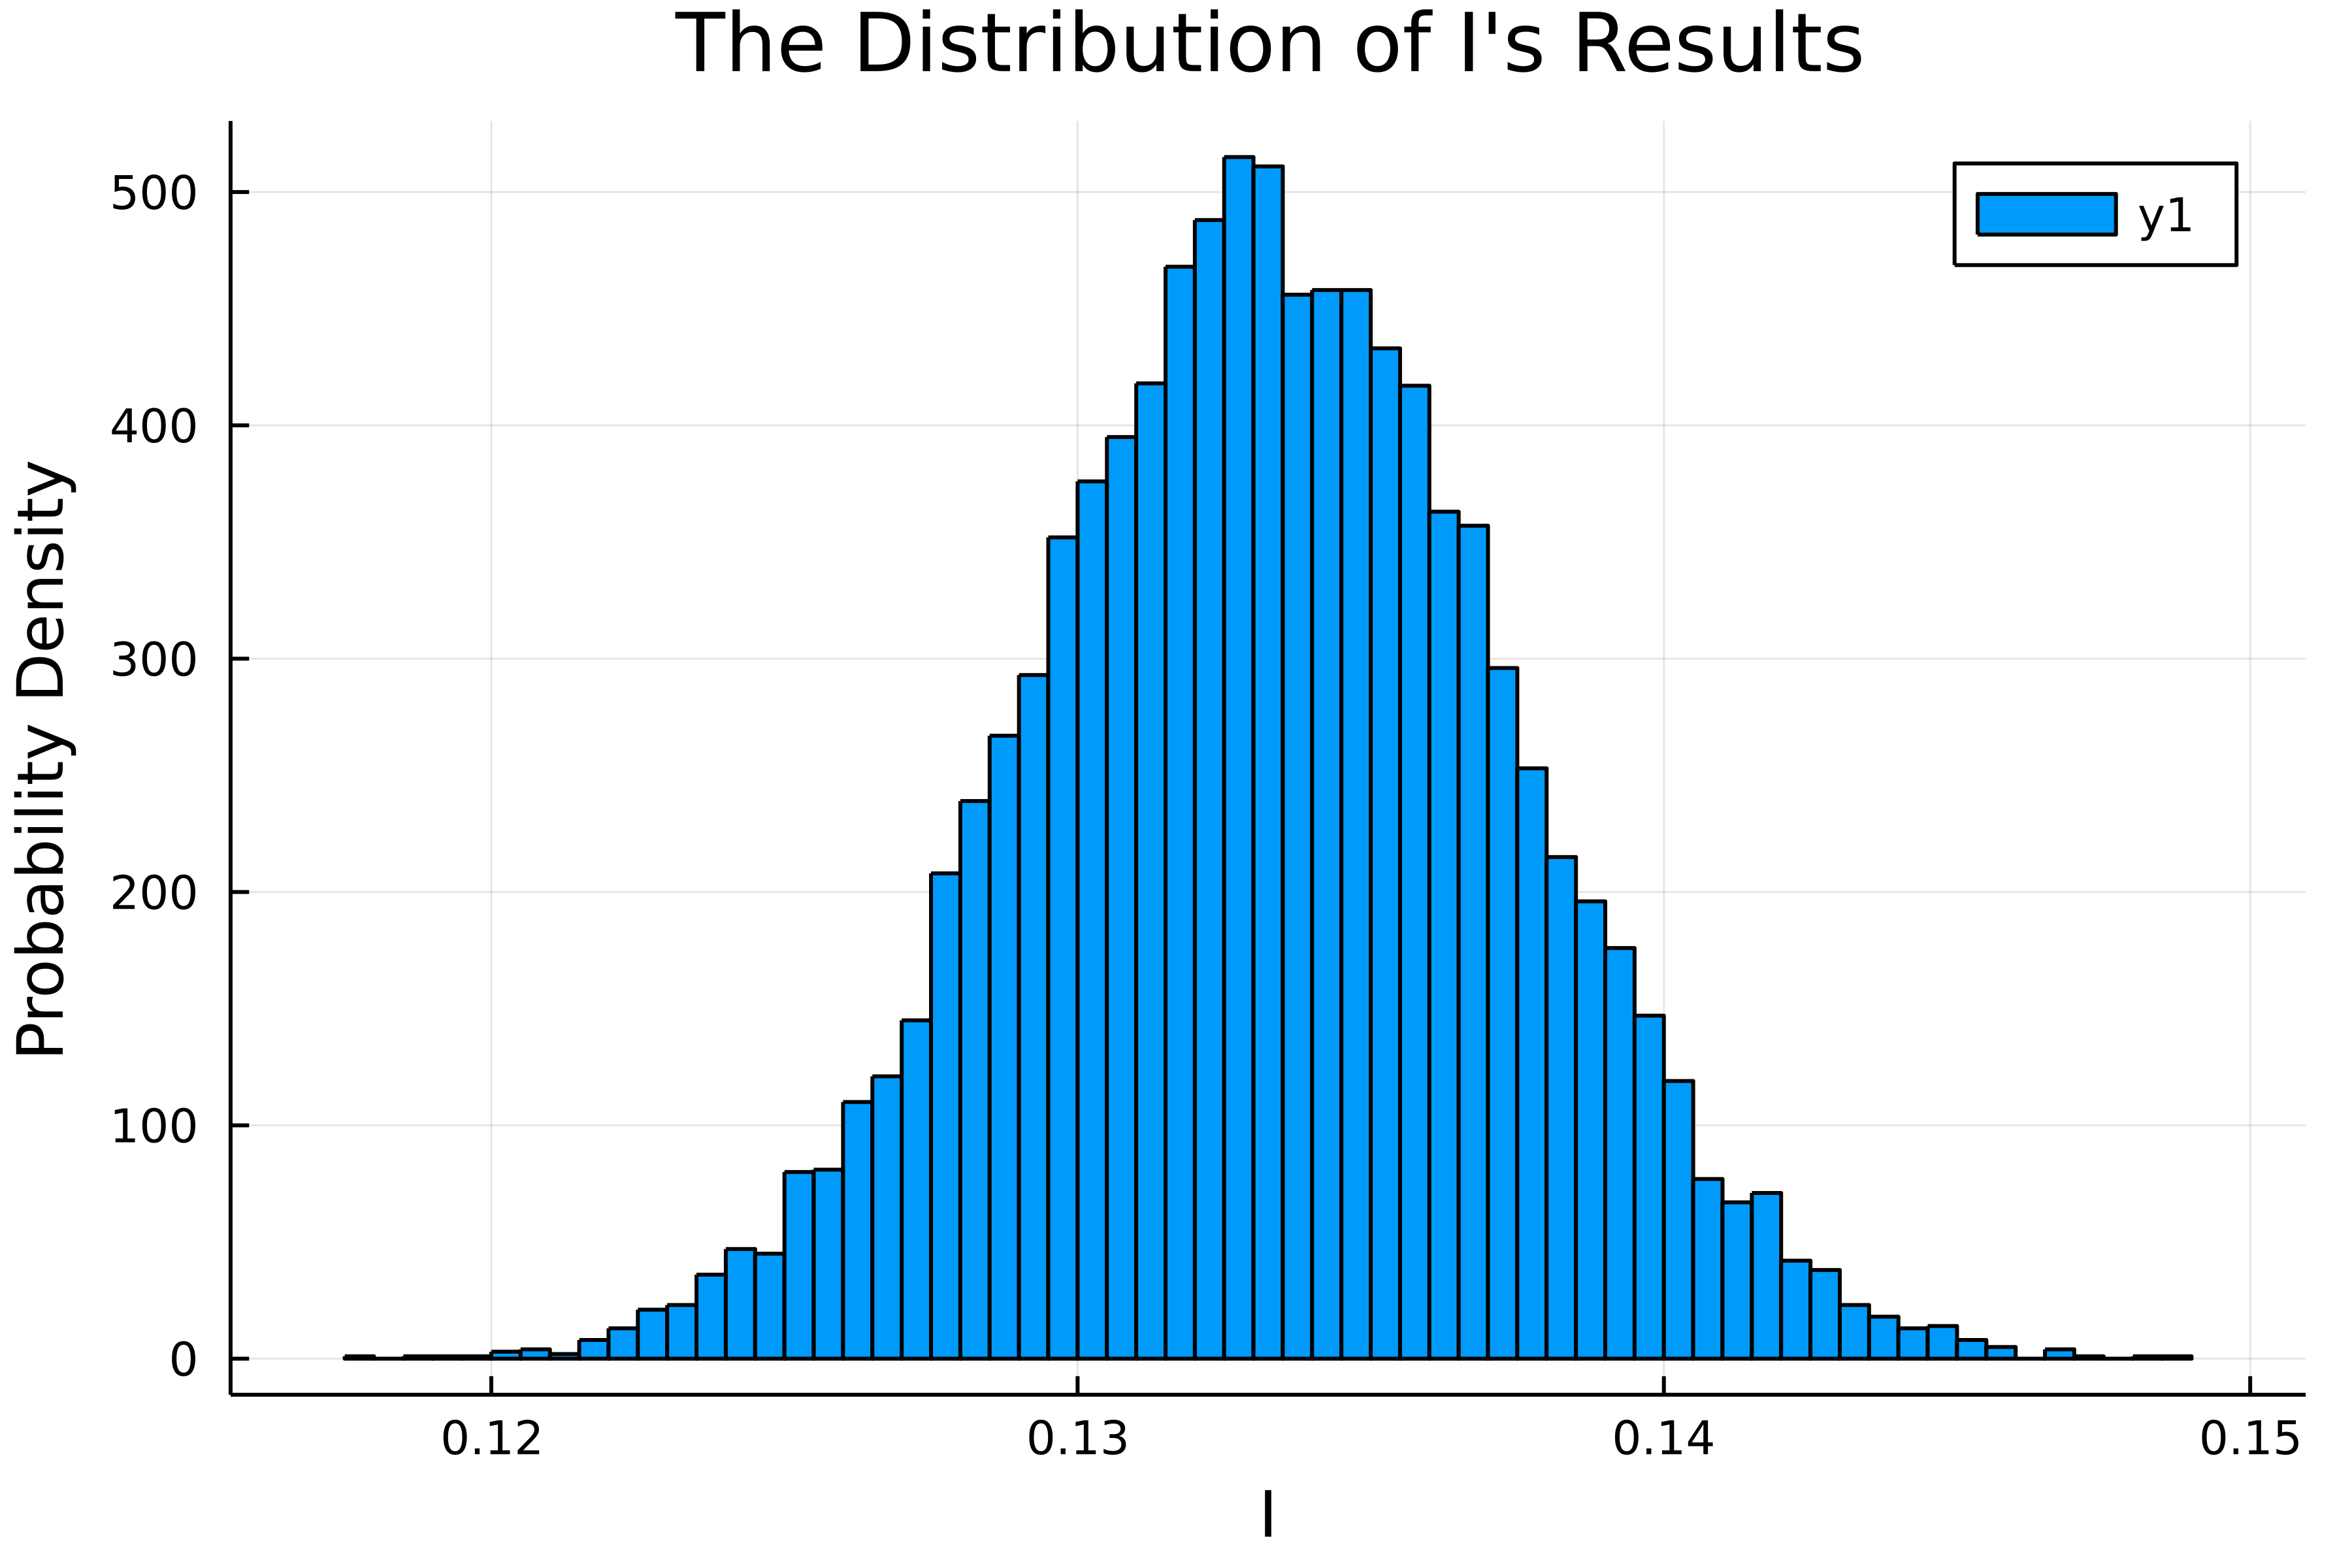
\includegraphics[width=\textwidth]{IHistogram.png}
		\label{fig:mesh1.1}
		\caption{}
	\end{subfigure}\par\bigskip 
	\begin{subfigure}[t]{0.8\textwidth}
		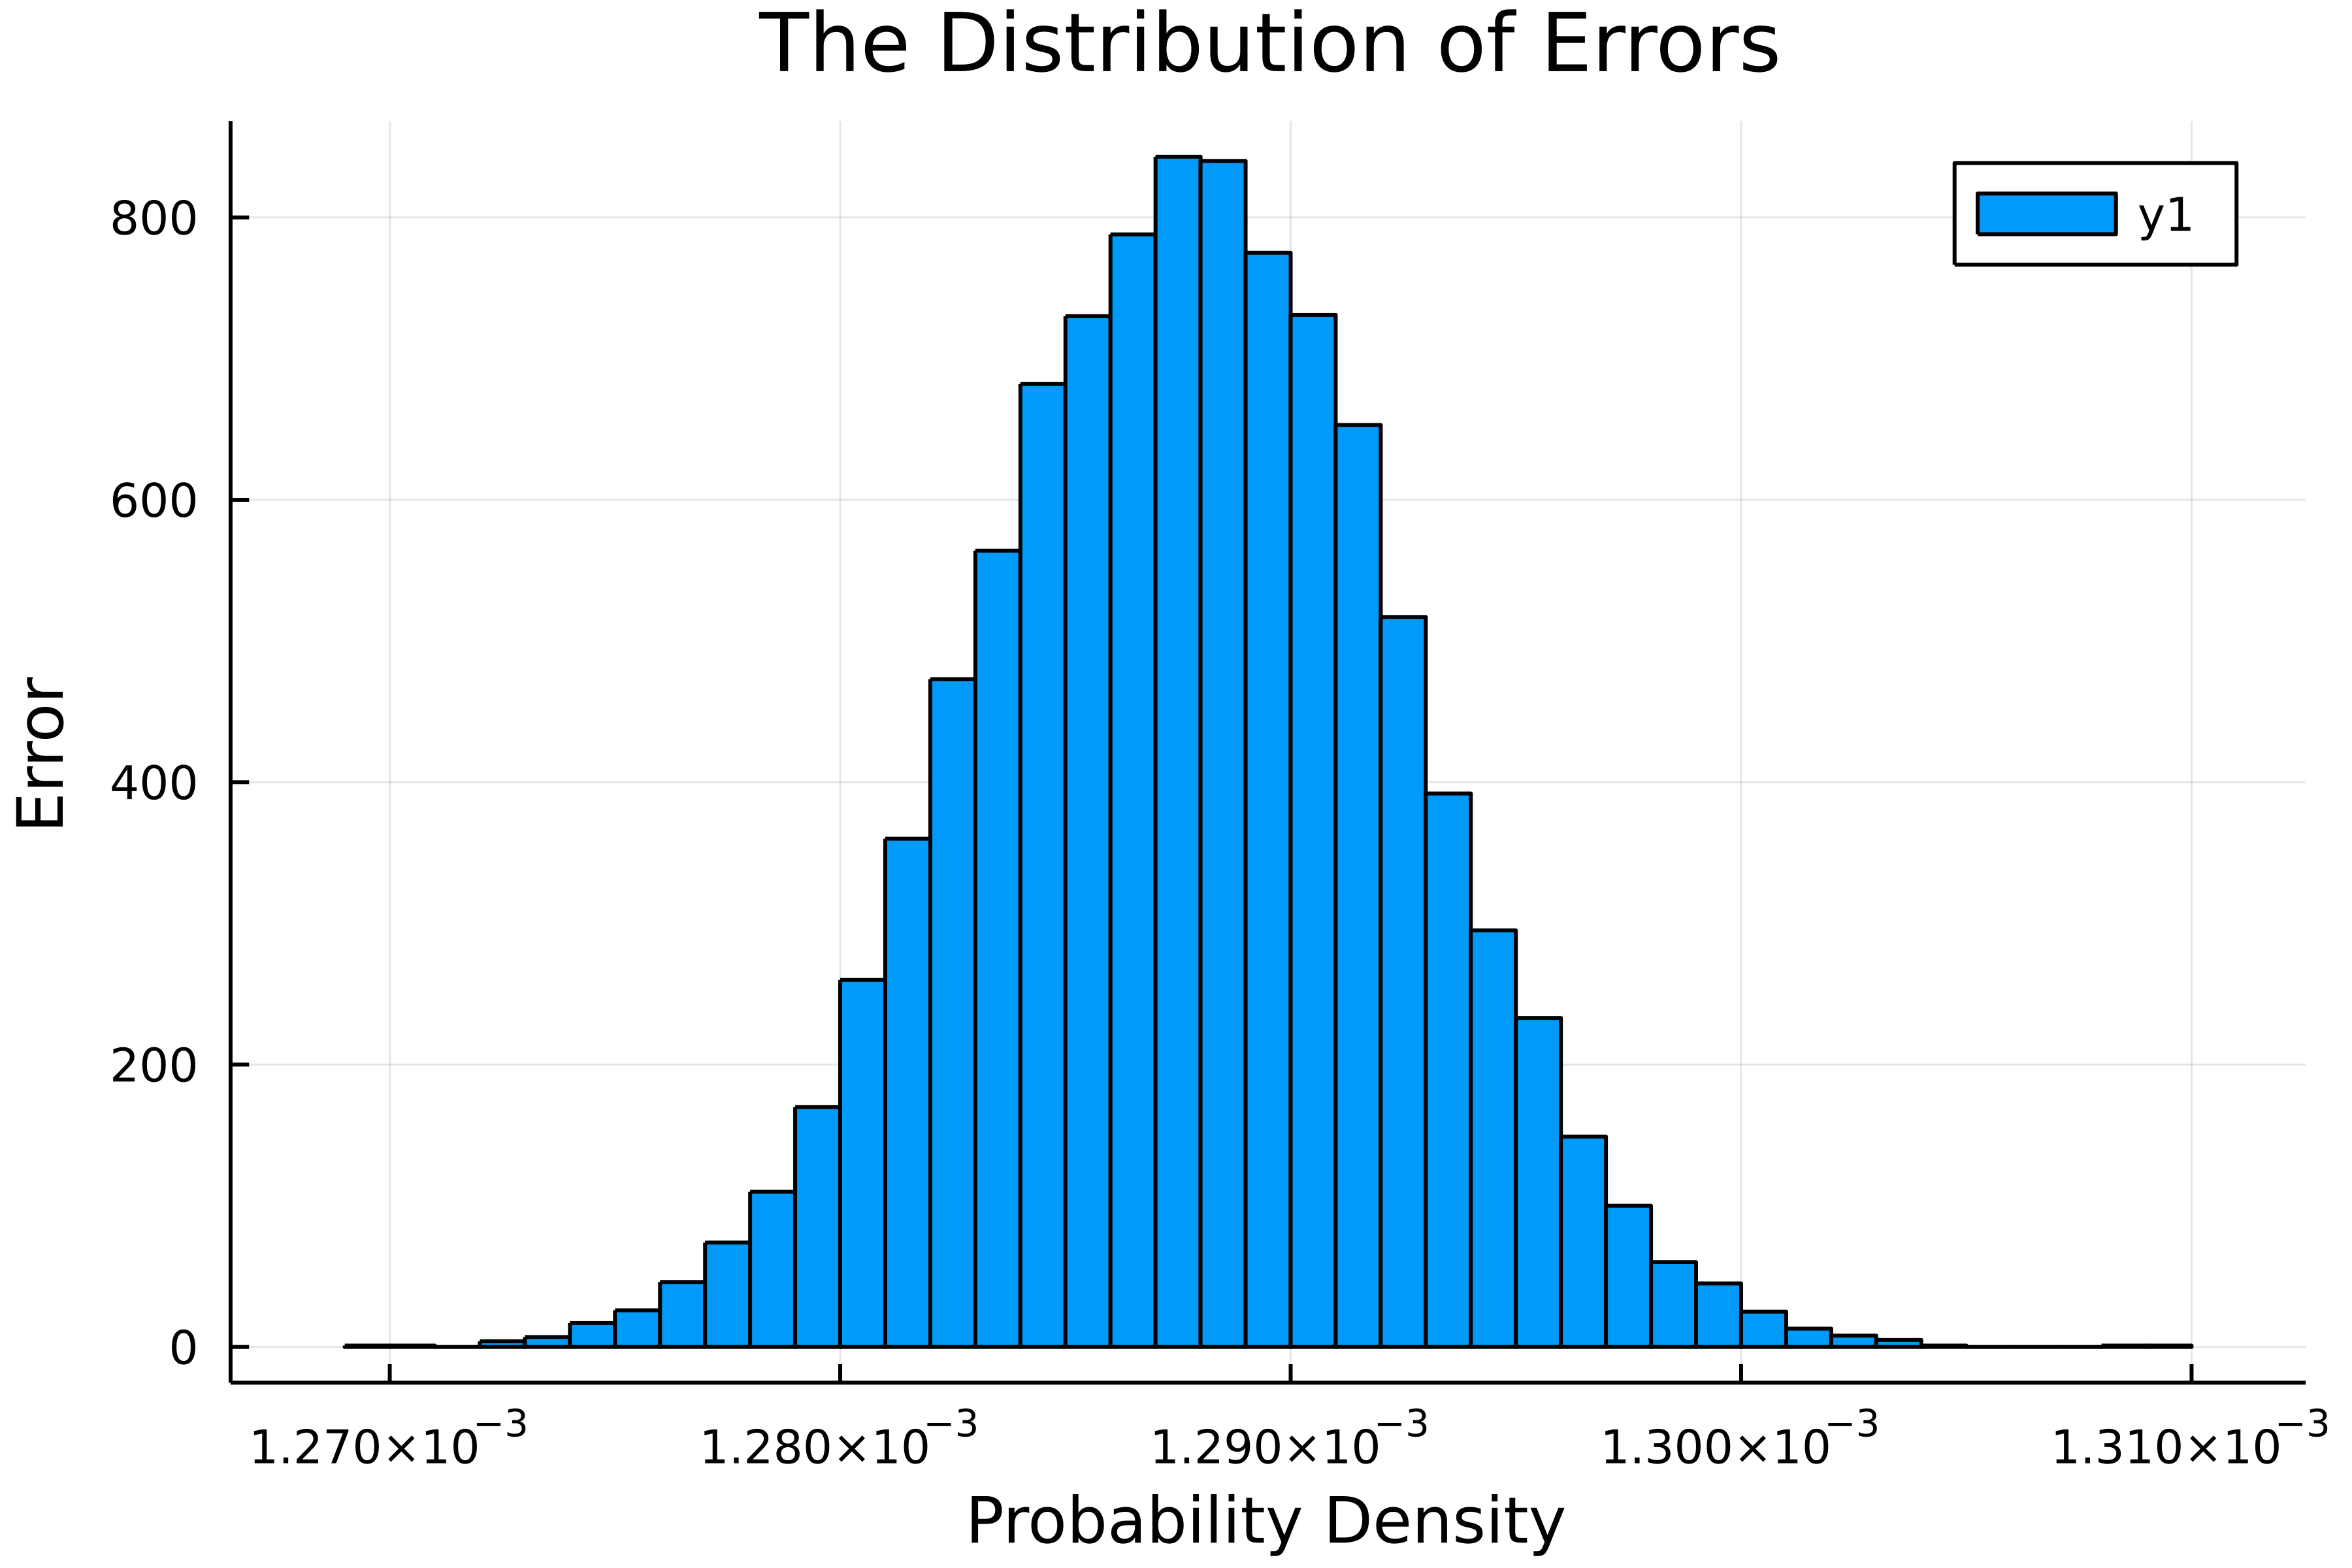
\includegraphics[width=\textwidth]{EHistogram.png}
		\label{fig:mesh1.2}
		\caption{}
	\end{subfigure}
	\label{fig:mesh1}
	\caption{Plots given for Exercise 7.2. R=1. Number of Samples=$10^{4}$}
\end{figure}
\part*{3. Exercise 8.1: Metropolis}
I used the Metropolis method in order to generate random numbers with a normal distribution. The relation between $a_{r}$ and dx(unit length of steps) are shown and further we come up with the auto correlation and the correlation length. 

\paragraph*{}
\begin{figure}[H]
	\centering
	\begin{subfigure}[t]{0.48\textwidth}
		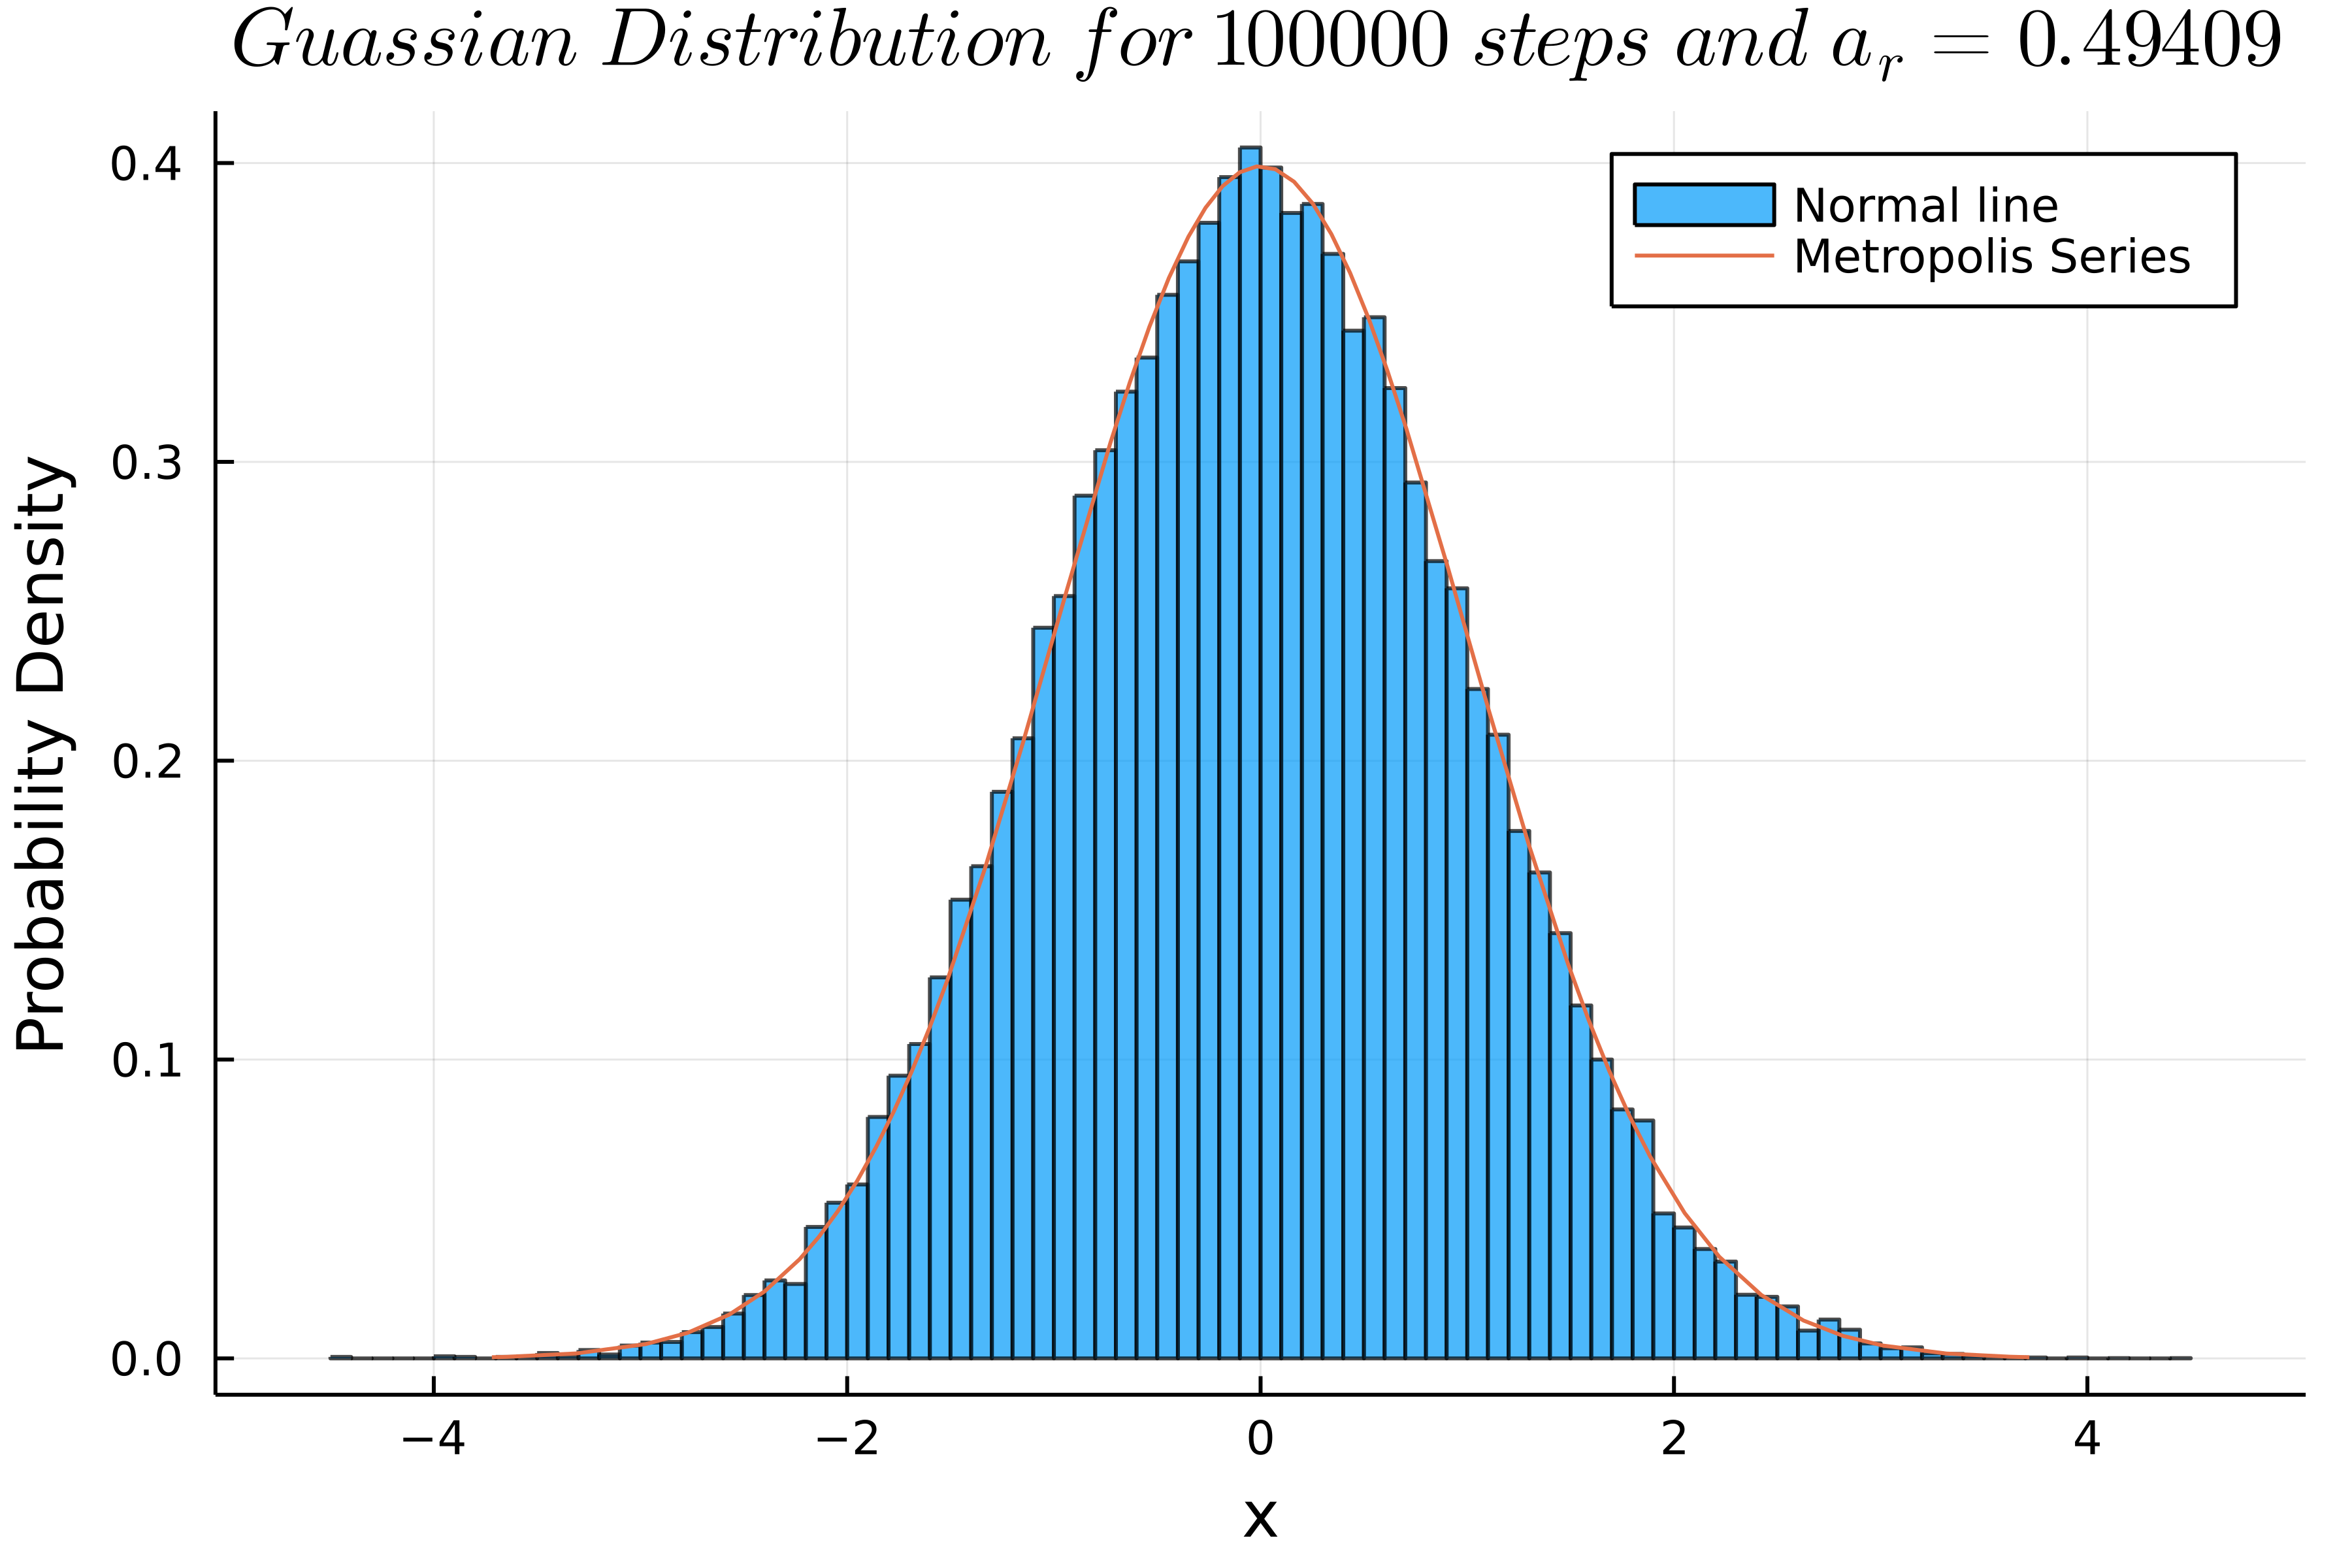
\includegraphics[width=\textwidth]{HistoPlot.png}
		\label{fig:mesh3.1}
		\caption{Number of steps=$10^{5}$ , dx=3.}
	\end{subfigure}\hfill
	\begin{subfigure}[t]{0.48\textwidth}
		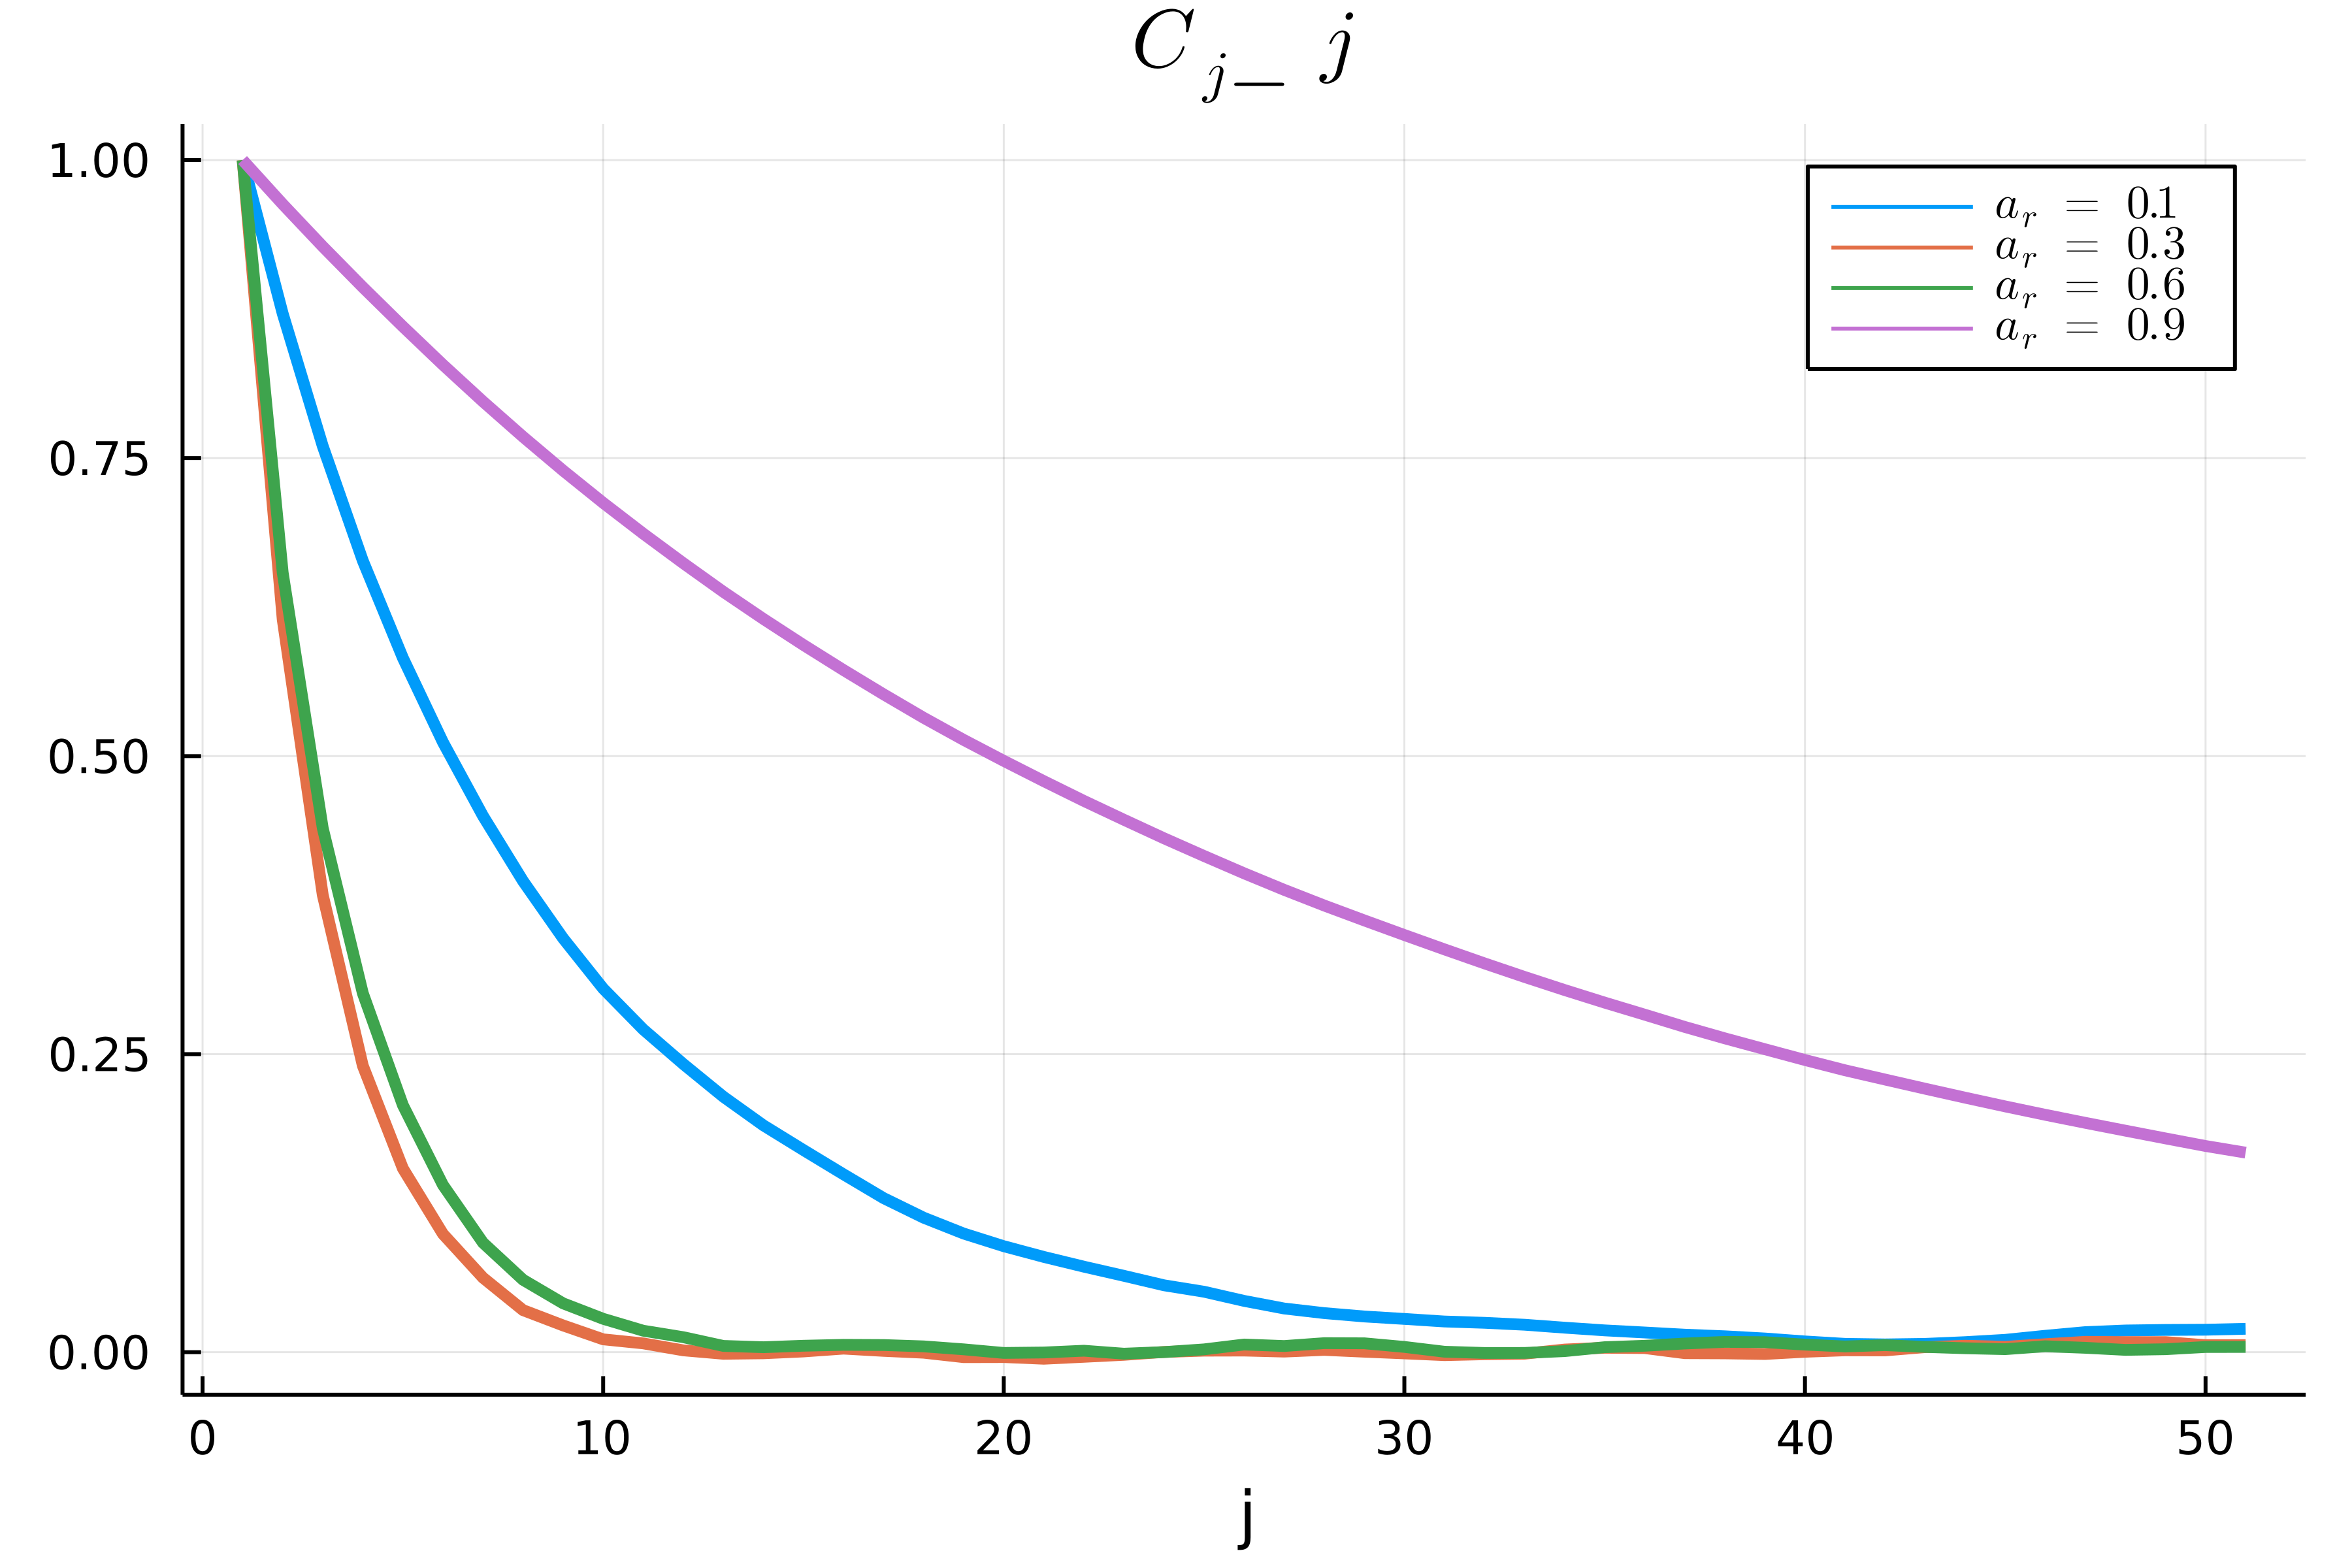
\includegraphics[width=\textwidth]{Cj_j.png}
		\label{fig:mesh3.2}
		\caption{dx are: 15.9, 7.95, 5.27, 3.88, 2.94, 2.2, 1.57, 1.03, 0.5. $a_{r}$=0.1, 0.2, 0.3, 0.4, 0.5, 0.6, 0.7, 0.8, 0.9. Number of Steps= $10^{5}$. }
	\end{subfigure}\hfill
	\begin{subfigure}[t]{0.48\textwidth}
		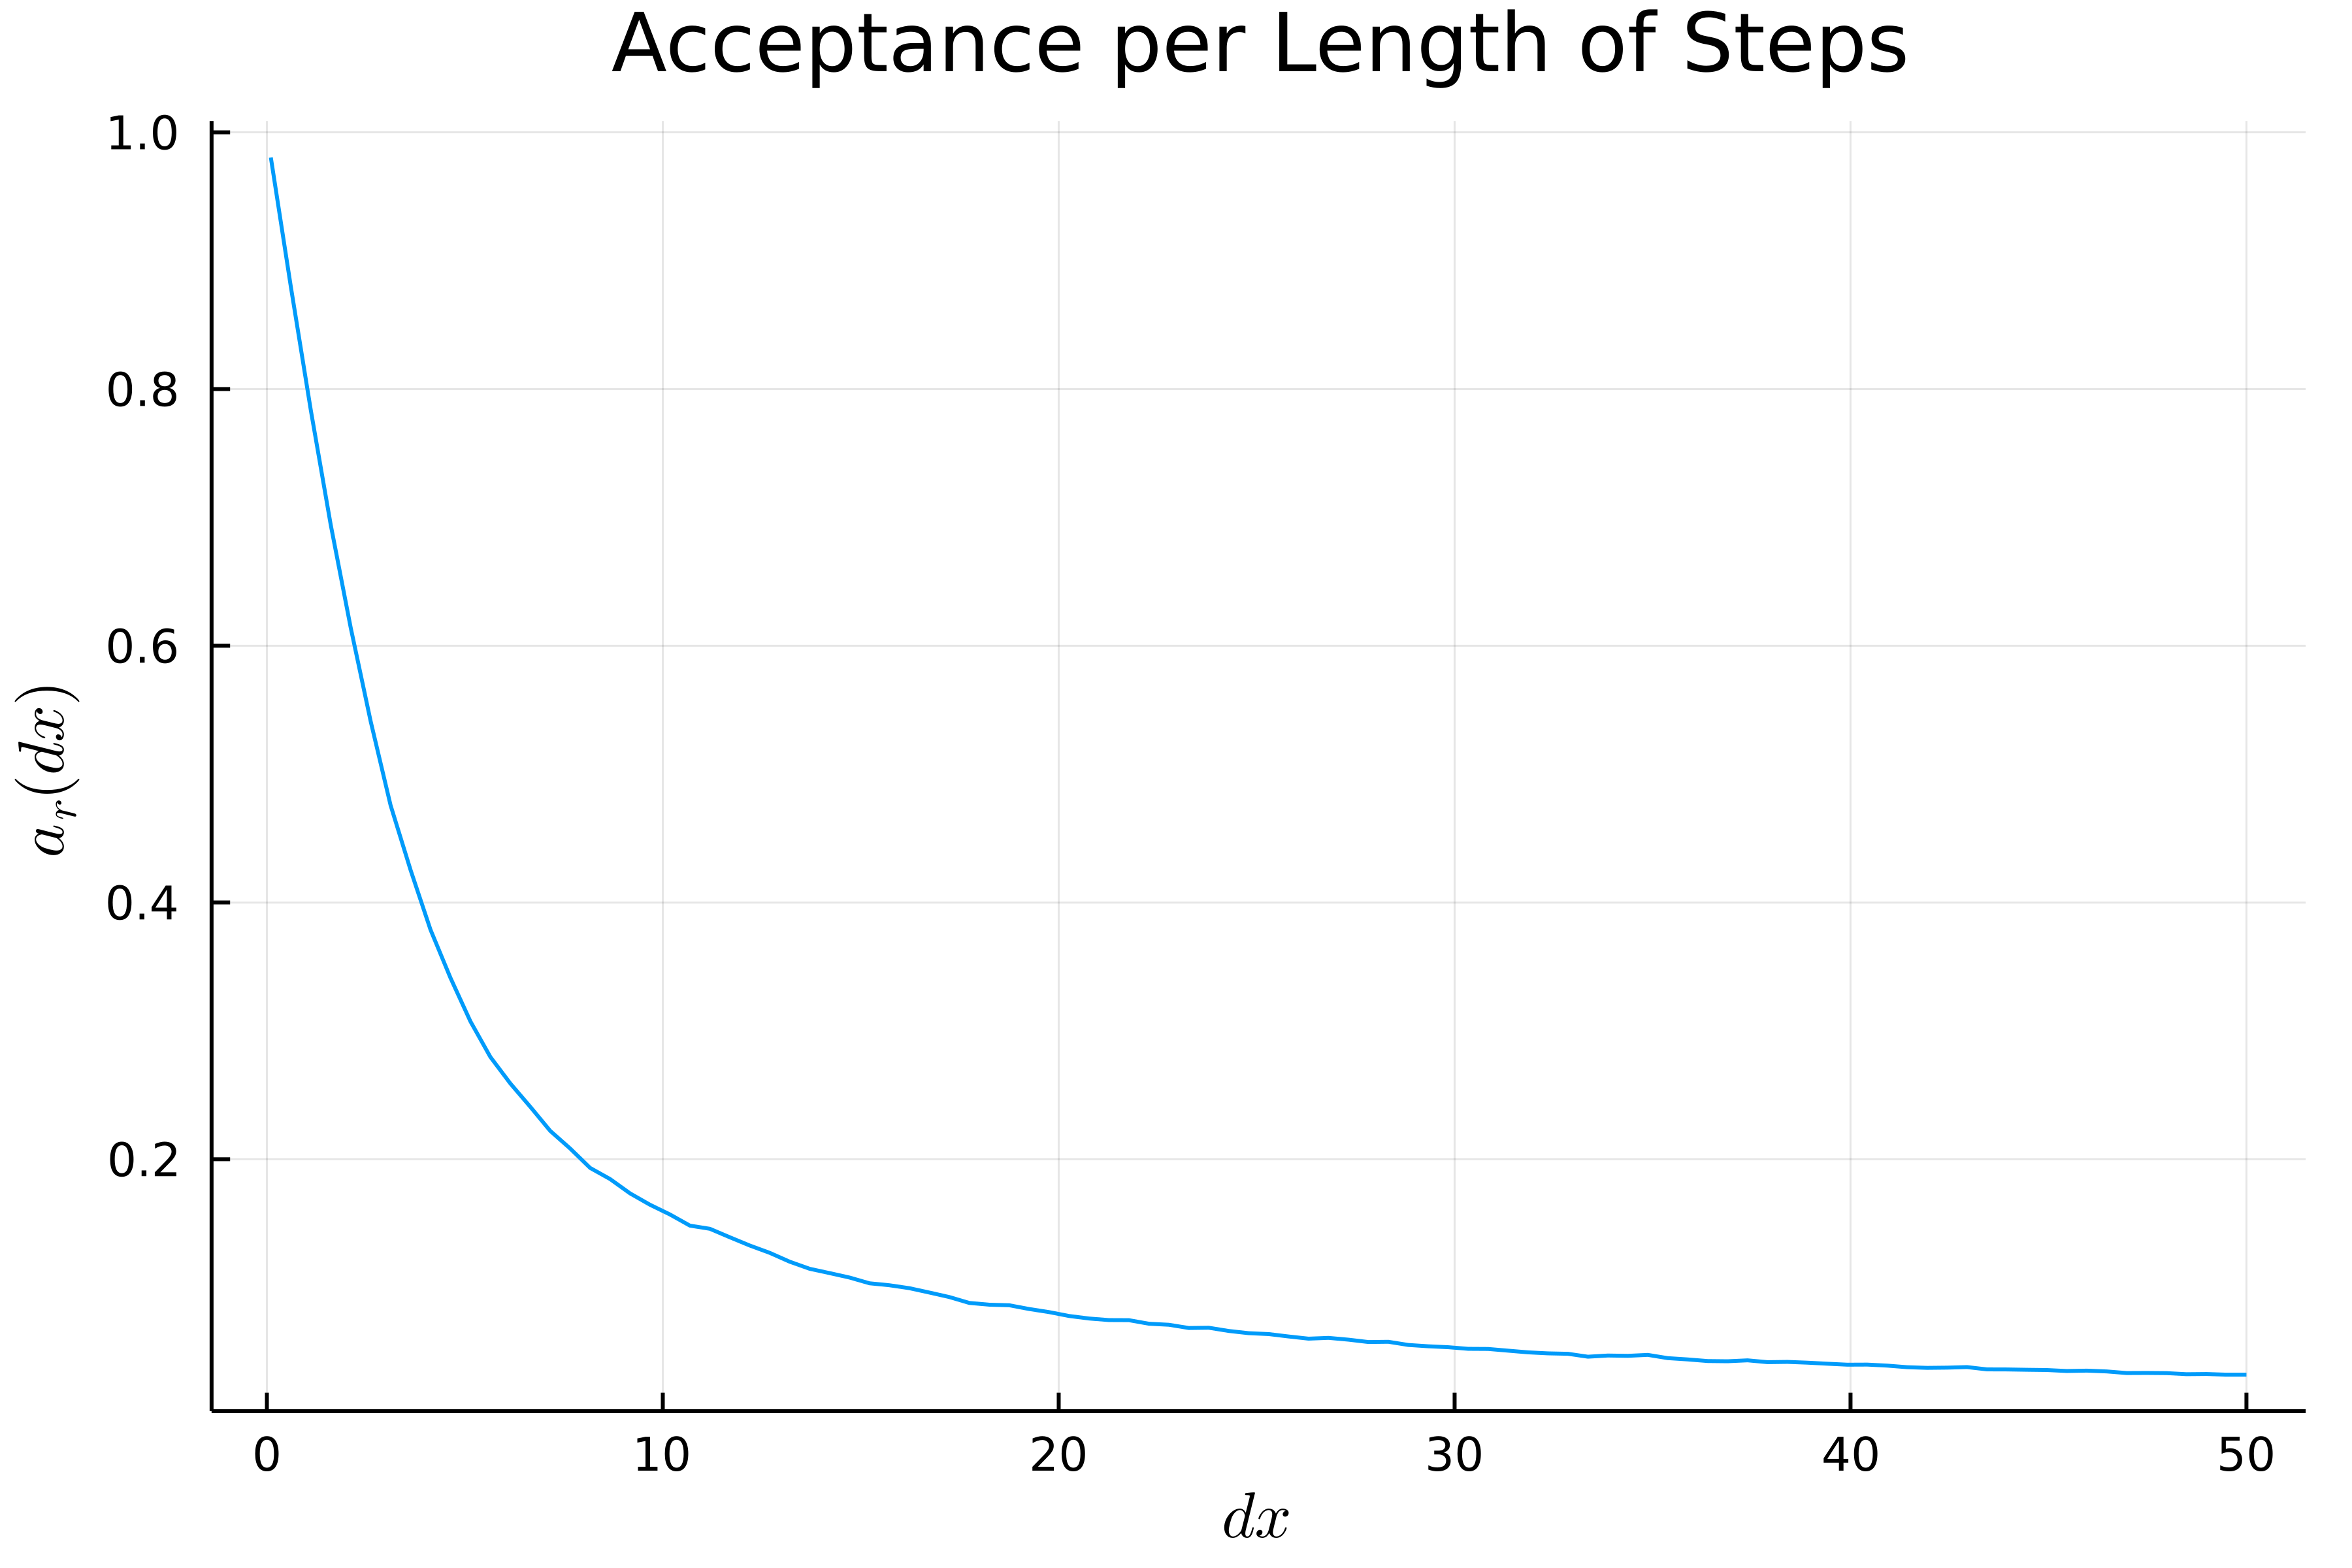
\includegraphics[width=\textwidth]{acceptance_ratio.png}
		\label{fig:mesh3.3}
		\caption{using the dx given in a list of steps from 0.1 to 50, a total number of 100 values. number of steps=$10^{5}$.}
	\end{subfigure}\hfill
	\begin{subfigure}[t]{0.48\textwidth}
		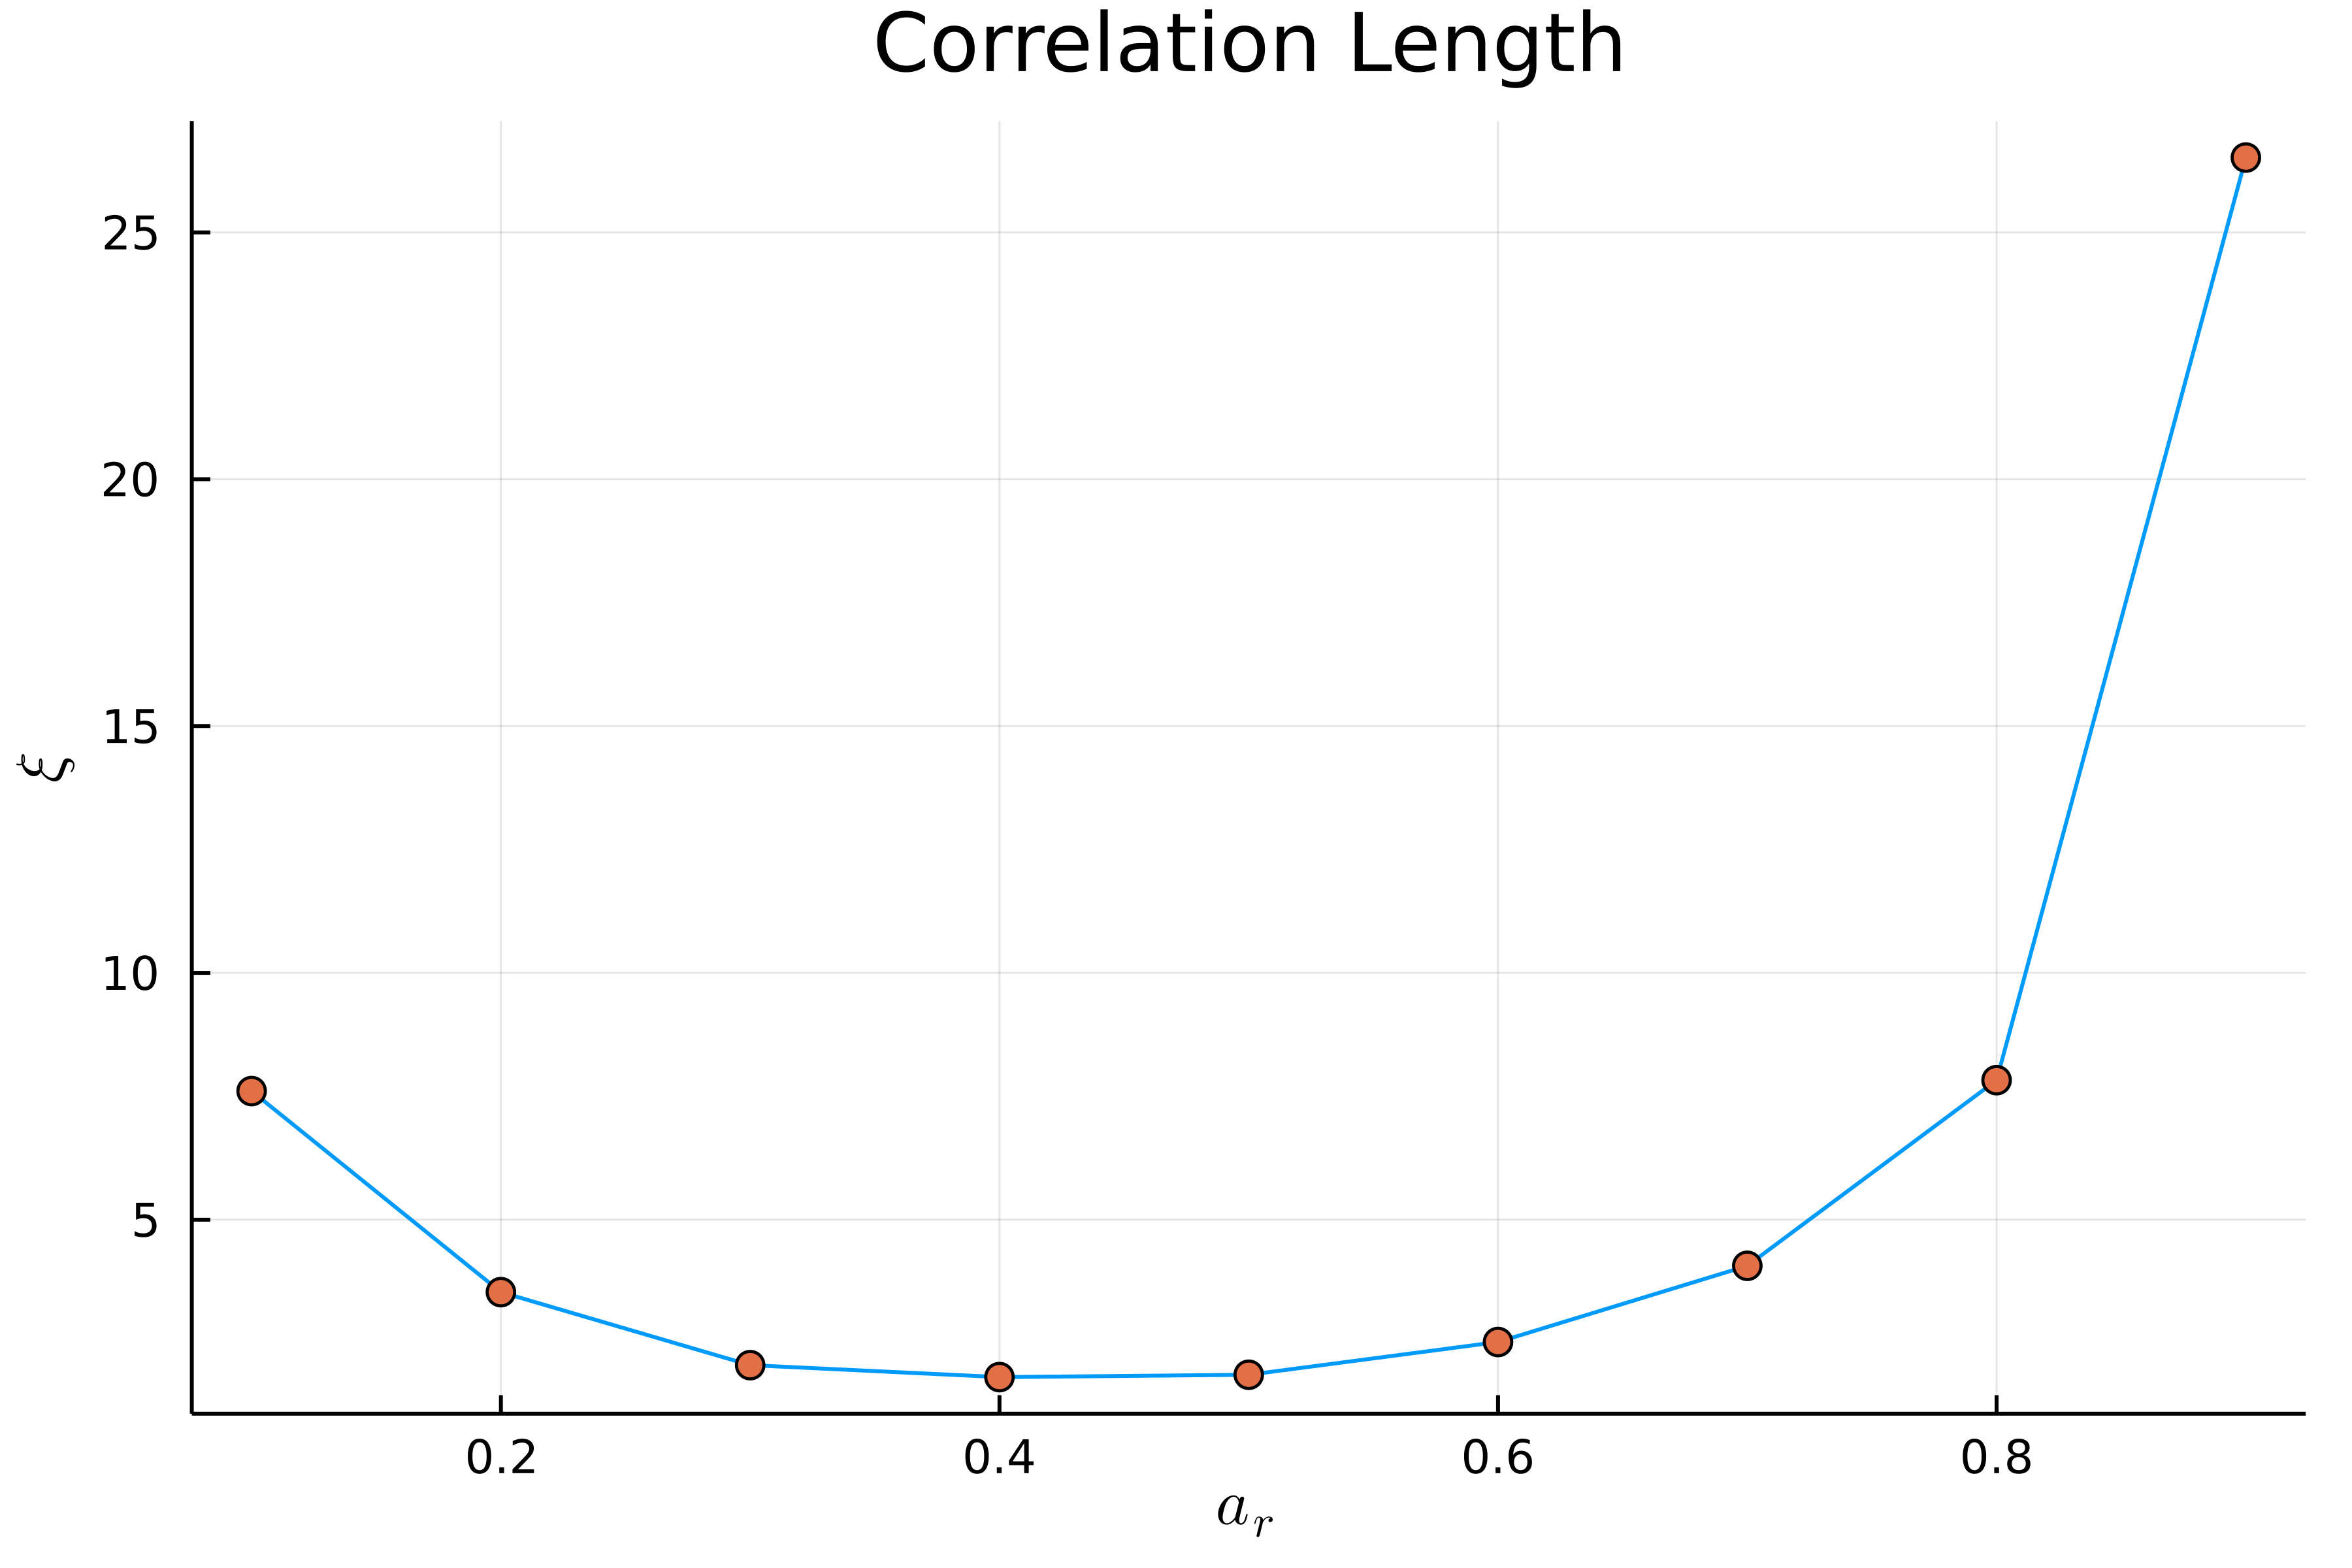
\includegraphics[width=\textwidth]{correlationLength.png}
		\label{fig:mesh3.4}
		\caption{Using the same data that were used in (b).}
	\end{subfigure}\hfill
	\label{fig:mesh3}
	\caption{Plots given for example 8.1. $X_{0}= 0$}
\end{figure}
The correlation Length is obtained by the equation given in the textbook.\\
    \textbf{refer to  \href{https://github.com/narges8k/computational_physics/tree/main/chapter6}{this link} to check the saved data.}
\end{document}